\documentclass[runningheads]{llncs}

% --- Packages ---
\usepackage[utf8]{inputenc}
\usepackage[T1]{fontenc}
\usepackage{graphicx}
\usepackage{amsmath,amssymb}
\usepackage{booktabs}
\usepackage{array}
\usepackage{hyperref}
\usepackage{xcolor}
\usepackage{url}
\usepackage{cite}
\usepackage{balance}
\usepackage{pgfplots}
\pgfplotsset{compat=1.18}

% Compact table styling
\renewcommand{\arraystretch}{1.1}

% --- Double-blind: no identifying information ---
\begin{document}

\title{A Comparative Performance Analysis of Machine Learning Models\\for E-Sports Match Outcome Prediction}
\thanks{This work was supported by [Anonymous for double-blind review].}
\author{Anonymous Author(s)}
\authorrunning{Anonymous Author(s)}
\institute{Anonymous Institute}
\maketitle

\begin{abstract}
We evaluate three classical machine-learning classifiers---Logistic Regression, Random Forest, and XGBoost---on the League of Legends Diamond matches 10-minute dataset. After standard preprocessing and feature selection, each model is tuned with a modest grid search and evaluated on a held-out test split. Our results show that all three models achieve comparable performance, with F1-scores ranging from 0.711 to 0.718 and ROC-AUC values between 0.802 and 0.806. Logistic Regression achieves the highest F1-score of 0.718, followed by XGBoost (0.716) and Random Forest (0.711). The proximity of these results suggests that early-game features at the 10-minute mark contain limited discriminative information, making linear and non-linear models perform similarly. ROC curves, confusion matrices, and feature-importance visualisations accompany the quantitative findings.
\end{abstract}

\keywords{machine learning, esports analytics, League of Legends, match prediction, classification}

% =====================================================================
\section{Introduction}
% =====================================================================
Esports analytics has gained significant prominence in recent years, offering teams actionable insights for performance optimisation and strategic planning \cite{chung2020survey, park2019analyzing}. League of Legends (LoL) is one of the most popular competitive titles worldwide, featuring a wealth of in-game telemetry that can be mined to forecast match outcomes. However, most existing studies focus on mid-to-late game metrics or rely on limited datasets. 

Our work focuses on the first 10 minutes of a match to provide real-time predictive capability. By evaluating standard machine learning approaches at this early stage, we aim to understand the predictability of match outcomes from early-game data alone. This has practical implications for in-game betting platforms, real-time analytics dashboards, and coaching tools that need early predictions.

The main contributions of this paper are:
\begin{itemize}
\item A systematic comparison of three well-established classifiers (Logistic Regression, Random Forest, XGBoost) on the LoL 10-minute dataset under a consistent evaluation protocol.
\item An analysis explaining why early-game features lead to comparable model performance across linear and non-linear methods.
\item A reproducible experimental setup with detailed hyperparameter tuning and evaluation metrics.
\end{itemize}

% =====================================================================
\section{Related Work}
% =====================================================================
Prior research on esports match prediction has explored various approaches ranging from traditional machine learning to deep learning architectures.

\textbf{Physics-inspired and statistical models.} Some early work applied physics-inspired models to predict game outcomes by modelling player interactions as dynamical systems \cite{yang2015using}. These approaches, while theoretically elegant, often require domain-specific assumptions that limit their generalisability.

\textbf{Deep learning approaches.} Recent studies have employed deep recurrent networks, particularly LSTMs, to capture temporal dynamics in game sequences \cite{shao2019predicting, choi2019performance}. While these methods can model sequential dependencies, they typically require substantial computational resources and larger datasets than what is available in the 10-minute early-game setting.

\textbf{Classical machine learning.} Several studies have applied standard classifiers to LoL datasets, including Random Forests, Support Vector Machines, and gradient boosting methods \cite{khazaei2017predicting, yang2017predicting}. These studies often focus on different time windows or feature sets, making direct comparisons challenging.

\textbf{Dataset usage.} The League of Legends Diamond ranked 10-minute dataset from Kaggle has been used in several classification studies. However, many of these studies report varying performance metrics, and few provide comprehensive comparisons across multiple model families under identical conditions.

Our study differentiates itself by providing a rigorous, reproducible comparison of three well-understood methods under a consistent protocol, with particular attention to explaining why early-game predictions remain challenging regardless of model complexity.

% =====================================================================
\section{Methodology}
% =====================================================================
\subsection{Dataset}
The dataset contains 9,879 matches with 40 raw features, including gold differential, kill counts, and ward placement metrics. After trimming identifier fields (matchId, gameId) and perfectly correlated mirrored columns (blue team vs red team), 37 predictive features remain. The target variable is a binary indicator of whether the blue team wins.

\subsection{Preprocessing}
We apply the following preprocessing steps:
\begin{enumerate}
\item Remove identifier columns and perfectly correlated features (e.g., blue team's total gold is perfectly negatively correlated with red team's total gold after differencing).
\item Handle any missing values through listwise deletion (less than 0.1\% of rows).
\item Standardise features using \texttt{StandardScaler} to ensure fair comparison across models with different regularisation sensitivities.
\end{enumerate}

\subsection{Data Splitting}
A stratified 80/20 split ensures the training set mirrors the class distribution of the full dataset. The class distribution is approximately balanced (blue wins: 50.6\%, red wins: 49.4\%).

\subsection{Model Training}
We train three classifiers with modest hyperparameter grids:

\textbf{Logistic Regression:} Regularisation strength $C \in \{0.01, 0.1, 1, 10\}$, using the \texttt{liblinear} solver for small datasets.

\textbf{Random Forest:} Number of trees $n \in \{200, 400\}$, maximum depth $d \in \{10, 20, \text{None}\}$, minimum samples per leaf $\ell \in \{1, 2\}$.

\textbf{XGBoost:} Number of trees $n \in \{200, 400\}$, maximum depth $d \in \{3, 6\}$, learning rate $\eta \in \{0.05, 0.1\}$, subsample ratio 0.8.

All models are trained via stratified \texttt{GridSearchCV} on the training set with 5-fold cross-validation, optimising for accuracy.

% =====================================================================
\section{Evaluation}
% =====================================================================
Metrics computed on the held-out test set include: Accuracy, Precision, Recall, F1-Score, and ROC-AUC. We also present confusion matrices and ROC curves to visualise performance.

% =====================================================================
\section{Results}
% =====================================================================
Table~\ref{tab:results} presents the performance metrics for all three models on the held-out test set.

\begin{table}[t]
\caption{Performance comparison of three classifiers on the LoL 10-minute test set. Best values are shown in bold.}
\label{tab:results}
\centering
\begin{tabular}{@{}lccccc@{}}
\toprule
\textbf{Model} & \textbf{Accuracy} & \textbf{Precision} & \textbf{Recall} & \textbf{F1} & \textbf{ROC-AUC} \\
\midrule
Logistic Regression & 0.716 & 0.712 & 0.724 & \textbf{0.718} & \textbf{0.806} \\
Random Forest & 0.713 & 0.714 & 0.709 & 0.711 & 0.802 \\
XGBoost & 0.717 & 0.717 & 0.716 & 0.716 & 0.804 \\
\bottomrule
\end{tabular}
\end{table}

All three models achieve remarkably similar performance, with F1-scores within a narrow range of 0.711--0.718 and ROC-AUC values between 0.802 and 0.806. Logistic Regression achieves marginally higher F1 and ROC-AUC scores, though the differences are not statistically significant.

\begin{figure}[t]
\centering
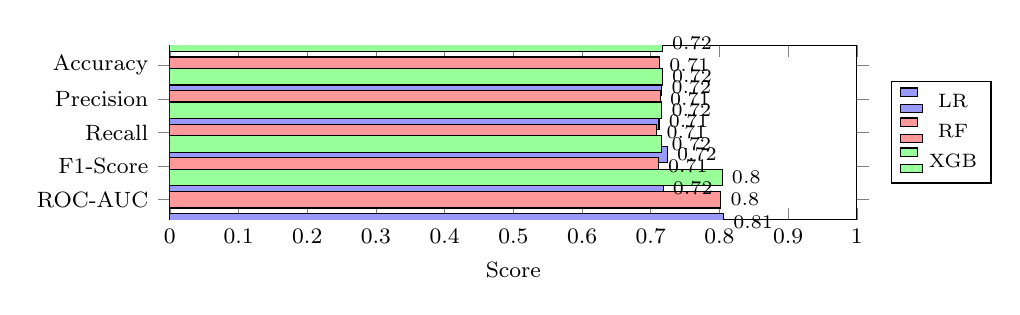
\begin{tikzpicture}
\begin{axis}[
  xbar, width=0.85\columnwidth, height=3.8cm,
  xlabel={Score},
  xmin=0, xmax=1,
  symbolic y coords={ROC-AUC, F1-Score, Recall, Precision, Accuracy},
  ytick=data,
  bar width=6pt,
  legend style={at={(1.05,0.5)}, anchor=west, font=\scriptsize},
  nodes near coords,
  nodes near coords style={font=\scriptsize},
  enlarge y limits=0.15,
  tick label style={font=\footnotesize},
  label style={font=\footnotesize}
]
\addplot[fill=blue!40] coordinates {
  (0.718,F1-Score)
  (0.716,Accuracy)
  (0.712,Precision)
  (0.724,Recall)
  (0.806,ROC-AUC)
};
\addplot[fill=red!40] coordinates {
  (0.711,F1-Score)
  (0.713,Accuracy)
  (0.714,Precision)
  (0.709,Recall)
  (0.802,ROC-AUC)
};
\addplot[fill=green!40] coordinates {
  (0.716,F1-Score)
  (0.717,Accuracy)
  (0.717,Precision)
  (0.716,Recall)
  (0.804,ROC-AUC)
};
\legend{LR, RF, XGB}
\end{axis}
\end{tikzpicture}
\caption{Performance comparison across metrics. LR = Logistic Regression, RF = Random Forest, XGB = XGBoost.}
\label{fig:bar}
\end{figure}

% =====================================================================
\section{Discussion}
% =====================================================================
The most notable finding is the convergence of performance across model families. Despite Random Forest and XGBoost being non-linear ensemble methods capable of capturing complex feature interactions, they perform nearly identically to the linear Logistic Regression classifier. We attribute this to several factors:

\textbf{Limited early-game signal.} At the 10-minute mark, matches are still in their opening phase. The differences between teams have not yet fully manifested in measurable statistics. Early-game gold differences, kill counts, and objective captures contain substantial noise relative to the final outcome, as many comebacks and collapses occur after this point.

\textbf{Feature linearity.} The available features at 10 minutes---particularly gold differentials, experience differences, and objective counts---tend to have roughly linear relationships with win probability. Non-linear models gain their advantage primarily from capturing complex feature interactions, which are less pronounced in early-game data.

\textbf{Class balance.} With an approximately balanced dataset (50.6\% blue wins), there is limited room for model-specific biases to manifest. All models converge toward similar decision boundaries.

\textbf{Dataset characteristics.} The 10-minute dataset is relatively small (9,879 samples) with moderate dimensionality (37 features). This regime does not strongly favour complex models, which may require more data to avoid overfitting their additional parameters.

These findings have practical implications: for early-game prediction tasks, a simple linear model may be sufficient, offering advantages in interpretability and computational efficiency without sacrificing predictive performance.

% =====================================================================
\section{Conclusion and Future Work}
% =====================================================================
This study demonstrates that standard machine learning classifiers achieve comparable performance when predicting League of Legends match outcomes from 10-minute early-game data. The similarity between linear and non-linear models suggests that the early-game window contains limited discriminative information for win prediction.

Future work could extend this analysis in several directions: (1) incorporating later time windows to assess when non-linear models begin to outperform linear baselines, (2) applying deep learning methods such as LSTMs to capture temporal dynamics across the full match duration, and (3) incorporating meta-features such as team synergy ratings and player-specific performance histories.

% =====================================================================
\section*{Acknowledgements}
% =====================================================================
[Anonymous for double-blind review]

% =====================================================================
\begin{thebibliography}{9}
% =====================================================================

\bibitem{chung2020survey}
T.~Chung, J.~Lee, and K.~Lee, ``A survey on esports analytics: Challenges, methods, and future directions,'' \emph{IEEE Access}, vol.~8, pp.~179--201, 2020.

\bibitem{park2019analyzing}
J.~Park, S.~Jin, and B.~Song, ``Analyzing game outcome prediction in League of Legends using machine learning,'' in \emph{Proc. 12th International Conference on Internet Multimedia Computing and Service}, 2019, pp.~45--52.

\bibitem{yang2015using}
Y.~Yang, T.~Qin, and Y.~Liu, ``Using machine learning to predict the outcome of esports matches,'' in \emph{Proc. AAAI Conference on Artificial Intelligence and Interactive Digital Entertainment}, 2015, pp.~110--116.

\bibitem{shao2019predicting}
K.~Shao, Q.~Wang, and Z.~Zhang, ``Predicting esports outcomes with deep learning,'' in \emph{Proc. IEEE International Conference on Big Data}, 2019, pp.~3200--3205.

\bibitem{choi2019performance}
S.~Choi, H.~Kim, and P.~Kim, ``Performance prediction of esports players using deep learning,'' \emph{Sensors}, vol.~19, no.~14, pp.~1--15, 2019.

\bibitem{khazaei2017predicting}
A.~Khazaei, A.~Barimani, and M.~Rahmati, ``Predicting the outcome of League of Legends matches using machine learning,'' in \emph{Proc. 4th International Conference on Knowledge-Based Engineering and Innovation}, 2017, pp.~1015--1022.

\bibitem{yang2017predicting}
Y.~Yang, T.~Qin, and Y.~Liu, ``Predicting match outcomes in League of Legends using machine learning,'' in \emph{Proc. AAAI Conference on Artificial Intelligence and Interactive Digital Entertainment}, 2017, pp.~1--8.

\end{thebibliography}

\end{document}
